(15, 3200 w)

Has the student carried out an evaluation?

Does the student present the results of the evaluation clearly and in a logical
manner?

Does the student explain the problems and difficulties found?

Does the student demonstrate an understanding and interpretation of results and
their significance?

Is there any critical evaluation of the project relative to the achievements of
related works?

Does the student present a personal reflection of what has been achieved and
not achieved in the project?

Has the student suggested future work?


\subsection{Simulation}
\label{sec:results}

\todo{open-source results}

\todo{list other hidden constants?}

\subsubsection{Inputs}

The experiments and their analysis can be repeated by following the
instructions in User Manual in Appendix \ref{sec:user_manual}. The result
datasets can be found in the open data set mentioned in
\ref{sec:intro:overview}.

Initially a baseline of inputs were chosen without any intentional constraints
on the environmental conditions. These inputs are shown in Table
\ref{table:input_data} and the full result data can be found in
\texttt{standard} directory in the data set.

\begin{table}
\begin{tabular}{ | l | l | }
  \hline
  Parameter & Value \\ \hline
  Time Limit & 1 000 000 \\
  Road network & with 6 locations, distances between 1-5 \\
  Passengers' expected fare & 20 \\
  Taxi's variable price range & 5-100 (integers) \\
  Taxi's benchmark price & 20 \\
  \hline
\end{tabular}
\caption{
  Simulation inputs
  \label{table:input_data}
}
\end{table}

The simulation was additionally run for control purposes, varying one input
parameter at a time. These runs are summarised in Table
\ref{table:inputs:control}, displaying the parameter in question and its
changed value, as well as the directory in the open data source where the
results are located.

\begin{table}
\begin{tabular}{ | l | l | l | }
  \hline
  Parameter & Value & Result Directory \\ \hline
  No changes & - & \texttt{standard} \\
  Benchmark price & 15 & \texttt{lower\_benchmark} \\
  Benchmark price & 30 & \texttt{higher\_benchmark} \\
  Taxi's price range & 5 - 20 & \texttt{lower\_range} \\
  Taxi's price range & 20 - 100 & \texttt{higher\_range} \\
  Time limit & 50 000 & \texttt{limited\_time} \\
  \hline
\end{tabular}
\caption{
  Control parameter changes
  \label{table:inputs:control}
}
\end{table}


\subsubsection{Summary}

In all simulation runs, the variable pricing approach performed significantly
better. The summary results are shown in Figure \ref{figure:results:summary}.

\begin{figure}
\begin{center}
  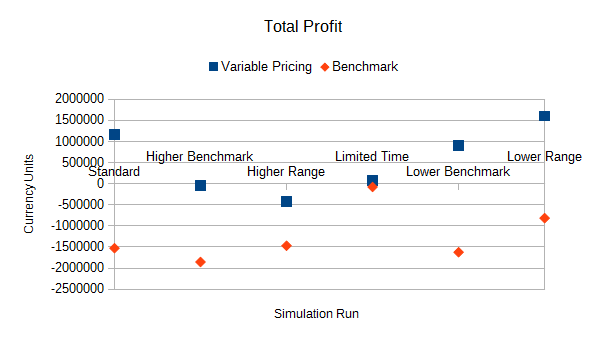
\includegraphics[width=\textwidth]{../figures/results_summary}
  \caption{
    Summary of Simulation Results
    \label{figure:results:summary}
  }
\end{center}
\end{figure}

Taxi using variable pricing earned a large profit in the simulation runs with
standard parameters, lower benchmark price and lower price range while the
fixed price taxi made large losses. The most profitable was the simulation
where the range of prices was limited to be lower than the expected price,
interestingly the fixed price taxi agent also performed better. The simulation
run with a limited time follow the same pattern but on a smaller scale
(varibale pricing 71382 profit / fixed pricing 74416 loss).

Neither pricing approach made a profit in the runs with a higher benchmark
price and a higher price range. The higher price range run was the only run
where the variable pricing agent made a considerable loss, and the profit
difference between fixed and variable pricing was smaller than in other
samples.

The fact whether a taxi agent made a profit or a loss is not at all important
for these results. The actual amount of profit/loss depends on the simulation
inputs which in this case were not created to resemble a realistic situation.

Emphasizing that in this simulation taxi's cost for waiting was 1 and time
limit was 1 000 000, the cost of a taxi not operating at all would be 1 000
000. It can be noticed that in all but one case the simulation with fixed
pricing generated larger losses than if the agent had been inactive, suggesting
that the reinforcement learning is not working to the taxi's benefit.

Nevertheless, these results strongly suggest that in identical conditions
having a choice to charge a varied range of fare prices is advantageous to a
taxi's profitability, and that Q-Learning can successfully be used for setting
the fare prices.


\subsubsection{Performance of Reinforcement Learning}
\label{sec:results:stats}

Analysis of variance was performed on each simulation's dataset (meaning that
benchmark and variable pricing runs were analysed separately). Detailed
simulation analysis is included in Appendices \ref{sec:data:standard},
\ref{sec:data:higher_benchmark}, \ref{sec:data:lower_benchmark},
\ref{sec:data:higher_range}, \ref{sec:data:lower_range} and
\ref{sec:data:limited_time}. This data is organised by simulation runs as
identified in Table \ref{table:inputs:control}, and each run has two parts --
variable pricing and benchmark.

All of the simulation runs show a statistically significant (95\% confidence)
increase of rewards for variable pricing taxi agents. The increase is
approximately 0.3 for the standard run, between 0.15-0.18 for all benchmark
price and price range runs, and a surprisingly high 0.75 for the run with
limited time.

However, data is less conclusive on the simulation runs with a fixed price.
Only the fixed price simulation with a higher benchmark price showed
statistically significant changes of rewards. Interestingly, this change was
negative, meaning that the agent actually got worse over time.

These results suggest that the taxi agent was successful at finding a policy
that increases the average reward when it can choose the price freely. 

However, questions about the effectiveness of the reinforcement learning
implementation are raised by the inconclusiveness and large losses of simulaton
runs with a fixed price, which is in sharp contrast to the success with
variable price simulations. Theoretically the agent should have learned the
actions that yield a higher profit by increasingly favouring travel between
more profitable locations. Could it be that the agent is good at selecting the
price but fails to select profitable locations? Could the agent's performance
be significantly improved by fixing this problem?
